%%%%%%%%%%%%%%%%%%%%%%%%%%%%%%%%%%%%%%%%%
% Simple Sectioned Essay Template
% LaTeX Template
%
% This template has been downloaded from:
% http://www.latextemplates.com
%
% Note:
% The \lipsum[#] commands throughout this template generate dummy text
% to fill the template out. These commands should all be removed when 
% writing essay content.
%
%%%%%%%%%%%%%%%%%%%%%%%%%%%%%%%%%%%%%%%%%

%----------------------------------------------------------------------------------------
%	PACKAGES AND OTHER DOCUMENT CONFIGURATIONS
%----------------------------------------------------------------------------------------
\documentclass[12pt]{article} % Default font size is 12pt, it can be changed here

\usepackage[font=small,labelfont=bf]{caption}

\usepackage{geometry} % Required to change the page size to A4

\usepackage{amsmath}

\geometry{a4paper} % Set the page size to be A4 as opposed to the default US Letter

\usepackage{graphicx} % Required for including pictures

\usepackage{float} % Allows putting an [H] in \begin{figure} to specify the exact location of the figure
\usepackage{wrapfig} % Allows in-line images such as the example fish picture

\usepackage{lipsum} % Used for inserting dummy 'Lorem ipsum' text into the template

\usepackage{verbatim} % Multi-line comments

\linespread{1.2} % Line spacing

\setlength\parindent{0pt} % Uncomment to remove all indentation from paragraphs

\graphicspath{{./Pictures/}} % Specifies the directory where pictures are stored

\usepackage{algorithm2e}

\usepackage{color}   %May be necessary if you want to color links
\usepackage{hyperref}
\hypersetup{
    colorlinks=true, %set true if you want colored links
    linktoc=all,     %set to all if you want both sections and subsections linked
    linkcolor=black,  %choose some color if you want links to stand out
}

%\usepackage{tocbibind} 	% add references to table of contents
\usepackage{amsmath}
\usepackage{amsfonts}
\usepackage{amssymb}
\begin{document}

%----------------------------------------------------------------------------------------
%	TITLE PAGE
%----------------------------------------------------------------------------------------

\begin{titlepage}

\newcommand{\HRule}{\rule{\linewidth}{0.5mm}} % Defines a new command for the horizontal lines, change thickness here

\center % Center everything on the page

\textsc{\LARGE \bfseries Using an Interactive Genetic Algorithm and Markov Chain to Compose Melodies Relevant to the User's Taste}\\[1.5cm]
\textsc{\large By}\\[0.5cm] % Minor heading such as course title
\textsc{\large Ben Gelb}\\[0.5cm] % Minor heading such as course title
\textsc{}\\[0.5cm]
{\large A Project Proposal Submitted in Partial Fulfillment of the Requirements for the Degree of Master of Science in Computer Science}\\[1.5cm] % Minor heading such as course title
{\large Supervised By Dr. Joe Geigel}\\[1.5cm] % Minor heading such as course title
%{\large Joe Geigel Department of Computer Science B. Thomas Golisano College of Computing and Information Sciences Rochester Institute of Technology Rochester, New York November 2010}\\[1.5cm]

%{ \large \bfseries Using an Interactive Genetic Algorithm and Markov Chain to Compose Melodies Relevant to the User's Taste}\\[0.4cm] % Title of your document
%\HRule \\[1.5cm]

%\begin{minipage}{0.4\textwidth}
%\begin{flushleft} \large
%\emph{Author:}\\
%Ben \textsc{Gelb} % Your name
%\end{flushleft}
%\end{minipage}
%~
%\begin{minipage}{0.4\textwidth}
%\begin{flushright} \large
%\emph{Supervisor:} \\
%Dr. Joe \textsc{Geigel} % Supervisor's Name
%\end{flushright}
%\end{minipage}\\[4cm]

{\large \today}\\[3cm] % Date, change the \today to a set date if you want to be precise

%\includegraphics{Logo}\\[1cm] % Include a department/university logo - this will require the graphicx package

\vfill % Fill the rest of the page with whitespace

\end{titlepage}

%----------------------------------------------------------------------------------------
%	TABLE OF CONTENTS
%----------------------------------------------------------------------------------------

\tableofcontents % Include a table of contents
\newpage % Begins the essay on a new page instead of on the same page as the table of contents 

%------------------------------------------------------------------------------------------
%	ABSTRACT
%------------------------------------------------------------------------------------------
\section{Abstract}
Music can be created by anything; it is the melody, which leaves a lasting impression. Simulating the process of evolution on a computer allows one to witness and impact the creation of melodies. I propose a technique to have the computer compose simple, but euphonic melodies by using a Markov chain and an Interactive Genetic Algorithm (IGA). A Markov chain is created from a user selected corpus, and is used to generate the initial population where individuals resemble musical segments the user enjoys. As a result, the initial population will consist of individuals relevant to the user's musical taste. Coupling the Markov chain with an IGA that allows the user to make modifications to each melody by re-ordering the notes, decreases the total number of generations the IGA needs to run for. Additionally, the type of interaction that the fitness function provides is much more engaging and fun for the user than previous approaches, which results in a decreased user burnout rate.

\newpage

%------------------------------------------------------------------------------------------
% INTRODUCTION
%------------------------------------------------------------------------------------------
\section{Introduction}
Artificial intelligence (AI) aims to create systems capable of solving problems in various domains. One such domain is melody composition. By simulating evolution on a computer, one is capable of witnessing and impacting the creation of melodies. However, "creating melodies which human listeners would appreciate has shown to be difficult with current AI techniques" \cite{Jensen}. Although melody composition can be modeled using mathematics, "it distinguishes itself by also involving human emotions and aesthetics, which are domains not fully understood and also difficult to describe mathematically" \cite{Jensen}. Thus, teaching the computer to compose appealing melodies proves to be a challenging problem as composers have their own, unique styles, which are not confined to existing rules. If composers cannot fully model the process when they create melodies then how can it be adapted to the computer? \\

Genetic algorithms (GA) have been around for decades and have proven "to be a powerful [tool] for searching in complex domains too difficult to tackle using analytical methods" \cite{Jensen}. While using this technique to compose melodies may appear to offer promising results, the biggest challenge will be the design of a fitness function. An automatic fitness function, which relies on mathematics to evaluate melodies is not dependent upon a human component, and therefore is more efficient as it directs "evolution towards pleasant melodies" \cite{Jensen}. However, this system will not fully capture the user's preferences as it is unable to translate subjective trends. A more suitable approach to capture the user's preferences is the utilization of an interactive fitness function, referred to as an interactive genetic algorithm (IGA). While less efficient and more strenuous on the user, the likelihood that the melody reflects the user's preference is much greater. By manually ranking each melody, the user will influence how future pieces sound, thus ensuring it aligns with the user's taste. Hence, composing a melody is not just about placing characteristics in their technically correct positions, it involves using emotion as a way to guide the composer through the complex domain that is music. \\

Coming up with a technique to algorithmically compose melodies that are relevant to the user's taste will require a couple of modifications to the typical IGA. One of the most influential components of an IGA is the generation of the initial population. The initial population serves as the IGA's starting point, and plays a large role in how many generations an IGA needs to run for before seeing decent individuals. In order to minimize the number of bad generations, subsets from a Markov chain are used to represent individuals in the initial population. The Markov chain is based on a user selected musical corpus. Typical IGA evaluations require a user to listen to a melody, and then provide it a score based on some internal, subjective rubric. It is a very linear process and doesn't truly capture how a user feels because all the IGA can see is a number. Instead, the IGA will require a user to listen to the melody, and then allow the user to actually play with and make modifications to the individual. Modifications include re-ordering the melody's notes. The types and number of changes made have different impacts on the individual's fitness score, and more importantly, provide the IGA with information on what the user liked and didn't like about the original individual. By using standard genetic operators, but altering how the initial population is generated and the type of feedback the user supplies, the  IGA should produce interesting, relevant, and unique melodies. \\


%------------------------------------------------------------------------------------------
% PROBLEM
%------------------------------------------------------------------------------------------
\section{Problem}
IGAs are prone to a fitness bottleneck when used for melody composition making it difficult to compose a compelling solution. Specifically, users experience fatigue when required to evaluate individuals over an extended period of time. Fatigue affects many stages of evolution resulting in under-evolved populations. Additionally, users are often inconsistent with their evaluations during the early and later generations \cite{Biles94}. It is certainly possible to create a compelling solution under these circumstances, however this requires a certain amount of finesse due to the amount of influence the bottleneck has on the design and quality of the system \cite{Biles94}. \\

%add in that humans cant hear multiple pieces of music simultaneously without ruining the way it sounds.

Typically, IGAs run for a limited number of generations as a user is unable to sit and evaluate millions of individuals in a reasonable amount of time. However, placing these constraints on an IGA limits how quickly a population evolves from generation to generation, often resulting in under-evolved individuals. Although the elimination of the human component can produce "intellectually stimulating noise" \cite{RBecker} by measuring the technical merit of an individual, it does not account for the user's musical preference, and lacks a compelling dimension, which can only be achieved through subjective feedback \cite{Biles94}. Furthermore, a large portion of the user's time is spent evaluating populations dominated by noisy data. This is largely influenced by the quality of the initial population and consistency in user evaluations. Inconsistent user feedback slows down the evolutionary process. Specifically, the amount of random noise found in early generations results in the user losing focus and assigning random scores \cite{Biles94}. This confuses the IGA and causes bad individuals to influence the next generation instead of being filtered out. \\

Fatigue is the only constant in this problem that is guaranteed to happen after the $n^{th}$ generation. It is a time dependent issue that poses a major threat to the IGAs performance. While limiting the size of the population and the number of generations reduces the amount of time the IGA runs, it also hinders the IGAs performance and the quality of the solutions. Early generations tend to be filled with noise representing random, unstructured individuals with a minimal number of relevant features. Even when a considerable amount of the noise has been filtered out, and the individuals start becoming decent, the rate of growth from one generation to the next is gradual. When time is of the essence it becomes essential to either replace the bottleneck or build around it. Therefore, it is imperative to design a system that accounts for human fatigue so that it does not dramatically alter the results. 

%------------------------------------------------------------------------------------------
% PREVIOUS RESEARCH
%------------------------------------------------------------------------------------------
\section{Previous Research}
Eliminating the fitness bottleneck prohibits the user from projecting their musical preference into the melody. Therefore, attempts have been made to minimize the bottleneck by studying the user's rating habits over a period of time \cite{Nao}. Neural networks (NN) have been able to replicate the user's taste to a degree allowing the IGA to run for a longer number of generations. While the auto-rater is able to maintain a consistency in its scoring, it is minimally successful in mimicking the user's taste, a result of an under-trained NN \cite{RBecker}. \\

The process of evaluating an individual typically require the user to listen to the melody and then assign it a score based on a linear scale representing the user's opinion of the overall piece. The inherent flaw is that even if a user enjoyed bits and pieces of the melody, the section that was enjoyed will typically be overlooked as the individual's evaluation is based on the entire piece, and not segment by segment. This type of evaluation is often the slowest to receive decent individuals due to its vague nature. \\

The concept of quality and quantity often go hand-in-hand in IGAs; supplying more consistent feedback results in better individuals. According to Biles, a population should be represented as a single continuous knowledge base \cite{Biles96}. In doing so, a unity among the population is achieved making evolution more fluid. The user is able to rank each gene in real-time ensuring that the good ones aren't overlooked. Additionally, the IGA knows specifically what the user liked and didn't like, and as a result, has reduced the number of bad generations in the beginning \cite{Biles96}. \\

An IGA needs a starting point, which can be generated randomly. However this can be problematic as it increases the amount of noise found in early generations, which in turn increases the amount of time the user is required to evaluate poor populations. The concept of randomly generating individuals is similar to pressing random keys on a piano and hoping for a pleasing melody. Surely an intriguing sound may occur on occasion, but relying on such an inconsistent approach is not ideal given the strict time constraints. \\

Seeding the initial population has been a promising approach given its ability to set boundaries in the otherwise infinite and random space that music offers \cite{Biles01}. Providing a sense of structure, even minimally, to each of the individuals reduces the amount of noise and decreases the gap between the starting population and the optimal solution. Determining the boundaries for generating the initial population are generally user defined or based on statistics. A common approach is to generate a Markov chain using user defined constraints, e.g. only minor chords. Doing this has shown to enhance the initial population's starting state. According to \cite{Shabda}, larger text often results in more choices at each transition, providing higher quality results. Evolution, even in its natural domain, is a slow process \cite{ToddWerner}. Any structure or guidance will have a positive impact on the quality of early generations.

%User burnout creates a fitness bottleneck making it difficult to find an optimal solution in a reasonable amount of time. This is because the IGA usually terminates before an optimal solution is found due to the limited population size and number of generations. Evolution is inherently a slow process due to the "forces of selection [being] very noisy and temporarily ineffectual" [http://www-abc.mpib-berlin.mpg.de/users/ptodd/publications/99evmus/99evmus.pdf]. In IGAs, decent solutions don't start appearing until generation X [CITE Biles]. Standard GAs don't need to worry about user burnout being , and as a result can run for millions of generations with extremely large population sizes. \\ 

%A lot of the past research has come up with ways to work around the fitness bottleneck by working it into the design of the system. The IGA needs to decrease the amount of time it takes to find an optimal solution given the strict termination requirements. This can be done by decreasing the number of generations it takes to start getting decent individuals. \\

%An auto-rater allows the GA to run for longer periods of time. It is a neural network that attempts to learn the user’s picking strategy in order to mimic it and replace the user. In doing so, the IGA is not confined to strict conditions and can run for longer periods of time. \\

%While the auto-rater is able to keep a consistency when evaluating, it isn’t able to actually mimic the user’s preferences. Due to the inherit time constraint in IGAs, the NN usually only has a small pool to draw from and ends up making poor evaluations due to minimal training time. One’s taste fluctuates with emotion [Find Citation]. The NN doesn’t truly understand the user’s preferences because we are unable to map emotions to equations at this time [Cite]. In the end, the autorater tends have a sub-optimal performance, while maybe mimicking the user's evaluation preferences X percent of the time [CITE]. \\

%IGA user interface (UI) optimizations have been made to speed up the evolution process. The UI is often implemented under the assumption that the user is ranking the individual on a scale. The user listens to a melody and assigns it a score, e.g. a number 1-100. This type of feedback supplies minimal knowledge to the IGA. It tells the system what the user thought of the melody as a whole compared to the others in the population. If a user liked certain segments of the song, but as a whole, hated it, then odds are those segments the user did like are going to be trashed. It also takes more time in the beginning to get a better generation going. \\

%Al Biles improved upon this by allowing the user to evaluate the population in real-time. Instead of his populations containing a number of melodies, his contains a single continuous melody, which is evaluated in real-time. The user ranks the melody by with either “g” for good or “b” for bad. This approach has reduced the number of generations needed for the populations to start becoming decent sounding [Find source verifying this]. According to Biles, good solutions don’t start appearing until generation X. \\

%The fitness function is not the only main contributor in an IGA’s success. Better initial populations tend to lead to future better populations [http://www.cameron.edu/~pdiaz-go/GAsPopMetric.pdf ]. An IGA terminates once it hits a specific number of generations. The more structure and starting knowledge the initial population has the less time that needs to be spent teaching it that. You want to limit the number so it can evolve more quickly. Better individuals produce better solutions and also reduce time spent in earlier generations weeding out large amounts of poor individuals. An IGA doesn’t have the luxury to run for thousands of generations like a GA can. With such a limiting factor, it is important to have to give it a jumpstart. \\

%Markov chains have been used to spawn the initial population and reduce the amount of randomness in the search space, which increases the probability that the selected traits will be closer to the user's taste, while simultaneously reducing the probability of bad individuals. \\

%The GA doesn’t need to use complex rules to determine the placement of notes and rhythm when creating a melody. Previous approaches had the user enter boundaries for the note for the Markov chain to create. But this doesn't speed up the rate to find an optimal solution. By building a Markov chain off of existing songs, many rules will already be intact since the songs already have their own rules embedded in them. \\

%It is important to determine the search space. Consider a song; it contains many parts, each building off the other. With each part containing a number of variables, the amount of time needed to find an appealing melody drastically increases. If a system is responsible for only creating 1 part of a song, the complexity decreases, thus increasing the likelihood of an appealing result. However, if the search space becomes too small, the chance of generating similar solutions drastically increases. It is important to determine the search space.

%------------------------------------------------------------------------------------------
% OVERVIEW
%------------------------------------------------------------------------------------------
\section{Overview}
\subsection{Interactive Genetic Algorithm}
An IGA is a search algorithm that has been influenced by Mendel's laws of classical genetics and Darwin's theory of evolution \cite{Jensen}. It has successfully solved problems in natural, social, and formal sciences, while sometimes generating unexpected and creative solutions. Formal IGAs structure themselves around the elements found in natural evolution, meaning there's a "population, diversity within the population, a selection mechanism, and genetic inheritance" \cite{Jensen}. The process begins by creating a pool of individuals to use as the starting point. Each individual, known as a genome, represents a chromosome. Genomes can be presented in many formats, but the most common one is a "set of binary integers such as 1001011" \cite{MIT}. Each member of the population is assigned a fitness score, which is a ranking that determines how fit it is. In an IGA, the fitness score is determined by a human, who evaluates each individual based on a personal, subjective rubric. Once the entire population has been evaluated, each individual is then passed to another function, which “selects individuals from the population to reproduce” \cite{MIT}. The selected chromosomes then crossover generating a set of children, which are used in the next generation. The children then have a chance of being chosen to undergo mutation in order to help keep the population diverse by randomly altering chromosomes. This process is repeated until the termination requirements are met.

\subsection{Markov Chain}
A Markov chain is a Markov process, which has a discrete state-space, and is used to represent a system that changes over time. It models transitions from one state to another for random, independent events, i.e., "the next state depends only on the current state and not on the sequence of events that preceded it" \cite{website:mc}. It works by creating a model from a collection of random variables. The model is a set, $S$, of states, $S=s_1,\ldots\,s_r$, and the transitional probabilities $P_{i,j}$ between the states. $P_{i,j}$ "is the probability that the Markov chain is at the next point in state $j$ given that it is at the present time point at state $i$" \cite{Ivo}. Thus, the Markov chain can be represented as $\Pr\left(X_{n+1}=x | X_n=x_n\right)$. The word "chain" is used to describe the output of this process because the results are often "chained" together. \\

This is similar to using a Markov chain to generate sentences where the output may not make complete sense, but grammar, sentence structure, and dialogue from the original text will be followed to a degree \cite{website:rose}. By setting a prefix size, a model can be built by gathering statistics about the frequency of which “words follow certain prefix groups of other words” \cite{website:rose}. For example, if $N$=2, the next generated words are based on the previous two words.

%------------------------------------------------------------------------------------------
% HYPOTHESIS
%------------------------------------------------------------------------------------------
\section{Hypothesis}
This research will focus on creating a system that can compose a compelling melody. In doing so, I will not only gain an understanding of how IGAs can be applied to subjective domains, but also a deeper understanding of music structure. While IGAs are often popular choices for solving creative problems, previous implementations require minimal human feedback due to  user fatigue. By altering the type of feedback the system requires, user fatigue becomes less of an issue and allows the IGA to arrive at an optimal solution faster than implementations that require the user to manually enter in a score. Minimizing the fitness bottleneck, and thus speeding up the rate an IGA converges, requires a system designed to exploit the most influential components in the evolutionary process; the fitness function and the initial population. \\

The first step is to alter the type of feedback required by the fitness function. The user becomes the composer and can make a limited number of adjustments to the melody. In doing so, I hope to improve upon the rate at which an IGA evolves, while also decreasing the amount of time it takes for undesirable individuals to die out. This is because the IGA learns what the user liked, didn't like, and ultimately, the preferred structure of the melody. Additionally, a Markov chain will be used to generate the initial population. It will be built off of user selected melodies with the goal of reducing the occurrence of weak individuals found in early populations. As a result, the individuals will have some structure embedded in them and contain a musical style that the user is already familiar with and likes. \\

%The type of feedback the user required by the user during evaluation needs to be changed. Allowing the user to become the composer and make a limited number of modifications to the melody increasing an IGA's rate of evolution, while decreasing the amount of time it takes for bad individuals to die out. The IGA learns what the user liked, didn't like, and ultimately, the preferred structure of the melody. \\ %Selection, even in natural evolution is a slow process. Bad individuals are able to slip through the cracks and infect future generations [http://www-abc.mpib-berlin.mpg.de/users/ptodd/publications/99evmus/99evmus.pdf]. \\


%I believe that there is a correlation between the rate at which an IGA arrives at an optimal solution (compelling melody) and the type of feedback supplied through the fitness function. By removing the earlier, more random generations, the IGA will have a better chance of creating an optimal solution. \\

%The fitness bottleneck isn’t going away; it must be considered in the design of the IGA and built around. One approach is to speed up the process of generating decent populations by using a catalyst. This can be done by implementing a new type of evaluation/rating/feedback system. One way to minimize the fitness bottleneck is to build the IGA around it. Since we don’t have enough time to run for the required number of generations, it is important to focus on reducing the amount of poor, random populations with inconsistent qualities among individuals in the earlier generations. No matter how intriguing a UI is, after an extended period of time most users will want to move onto doing something new [Find citation about interest levels!]. 

%In allowing the user to make a limited number of changes to the melody, the IGA can see what the user liked, didn’t like, and the ultimately, the ideal structure of the melody. This will lessen the amount of time it takes for bad individuals from each population to die out. Selection, even in natural evolution is a slow process. Bad individuals are able to slip through the cracks and infect future generations [Cite]. However, bad individuals should be given a fair chance. If they can be fixed with re-ordering then they should be able to. 

%The IGA needs to generate better populations quicker. Can do this by intelligently creating the solution space so it has more structure. Use a Markov chain where the chain is built off of sounds the user is already familiar with and likes. Markov chain with user selected melodies.

%Modify UI to allow the user to evaluate the individual in a different way. Let user make modifications to the melody to inflict their preference. This should speed up the process of generating better populations because the IGA can now see what the user liked, didn’t like, and ultimately how the user would’ve preferred the melody to sound. Additionally, it puts the user in control of mutation. 

%IGAs do a much better job at composing compelling melodies than GAs, but still have areas that can be improved. It is known that using an influencer when spawning the initial population provides better individuals than relying on a random initial population. By modifying the UI and type of feedback, there will be a reduction in the number of generations it takes for IGAs to start producing decent individuals 

\subsection{Questions}
Will this keep the user engaged and reduce burnout? How many individuals should be displayed at once? How many individuals from the generation should the user be required to listen to? Is it possible to bypass ones that are very similar? How many adjustments should the user be allowed to make per individual? How many influencers should be used?

%----------------------------------------------------------------------------------------
% SYNTHESIS
%%----------------------------------------------------------------------------------------
\section{Synthesis}
\subsection{System Architecture}

%\begin{figure}[H]
%\center{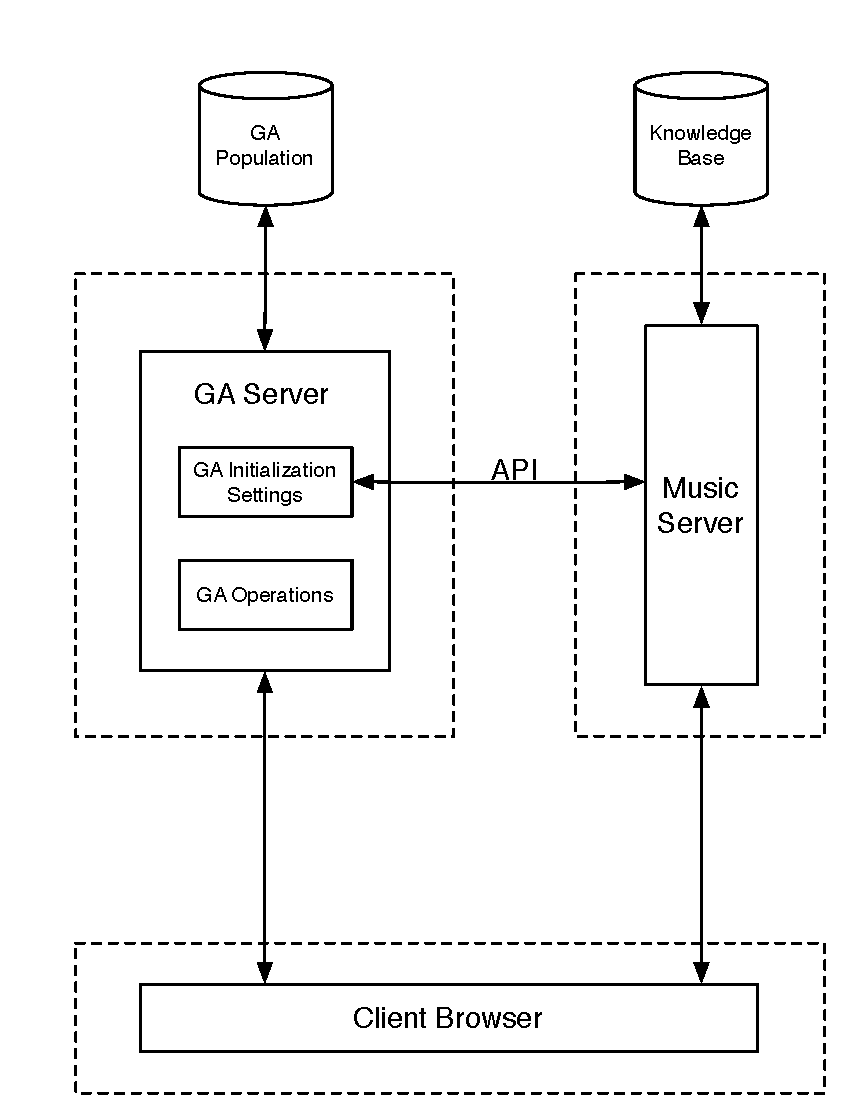
\includegraphics[width=.7\linewidth]{Pictures/server_architecture.pdf}}
%\caption{System Overview}
%\label{fig:sys_overview}
%\end{figure}

The IGA is composed of three parts: a web-server (music server), a GA, and a redis database. The music server is responsible for interpreting and directing web requests. It is composed of various endpoints, some of which are RESTful and others which are used to progress the state of the GA. The GA is a standalone library, which can be run independently from the music server.  The redis database is responsible for caching user options, individuals from each generation, and song features from the original MIDI file, which includes the notes, chords, and durations as well as the Markov chain generated for the specific song. \\

User experience (UX) is a crucial factor in the success of this system. Traditional software GUIs are not only tedious to program, but can’t match the seamless experience provided by a web-application. Using the web triforce (HTML5, CSS3, and JavaScript) allows for a significant level of control over the UX and user interface (UI), which in turn are responsible for user burnout.

\subsection{Breakdown of Music Server}
The music server acts as a middle-man between the GA and redis. The RESTful component of the music server supports GET and PUT requests for querying and updating a population from any generation and speicifc individuals. As a result of this architecture, the GA can be written in any language as long as it sends the required information to the music server about its current state. The RESTful endpoints can be seen below. 

\begin{enumerate}
\item Generate a population 
\begin{itemize}
\item GET /spawn
\item URL query parameters:
	\begin{itemize}
		\item psize (population size)
		\item isize (individual size)
		\item gsize (number of generations)
		\item mcsize (Markov chain size)
		\item mcnodes (Markov chain number of nodes)
		\item artist
		\item song
	\end{itemize}
\end{itemize}
\item All individuals and their metadata up until the current generation
\begin{itemize}
\item GET /population
\end{itemize}
\item All individuals and their metadata for the requested generation
\begin{itemize}
\item GET /population/:generation
\end{itemize}
\item Metadata for the requested individual
\begin{itemize}
\item GET /population/:generation/:id
\end{itemize}
\item Update a specific piece of metadata for an individual
\begin{itemize}
\item POST /population/:generation/:id
\item URL query parameters:
	\begin{itemize}
		\item key (fitness, notes, artist, song)
	\end{itemize}
\end{itemize}
\end{enumerate}

%\begin{figure}[H]
%\center{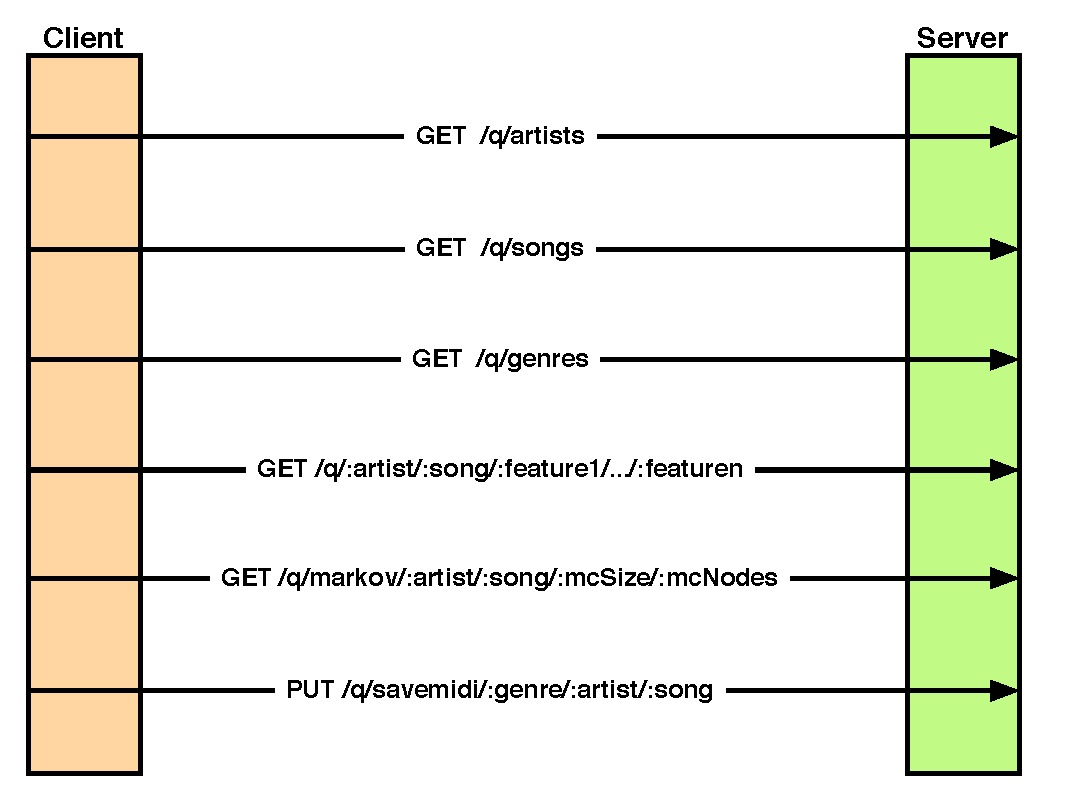
\includegraphics[width=.8\linewidth]{Pictures/rest_api.pdf}}
%\caption{REST API}
%\label{fig:rest_api}
%\end{figure}

\subsubsection{Extracting Metadata from MIDI files}
Music21, a Python library for music analysis from MIT \cite{website:music21} is used to decode the MIDI file and convert the low-level structure into a human-readable format. A sample of converted output can be seen in Table~\ref{midi_encode}. For this project, the file's notes, chords, and durations are extracted and stored in redis.


\begin{center}
\captionof{table}{Components of a Music21  Stream}
  \begin{tabular}{|l|}
    \hline
	{0.0} music21.stream.Part object at 0x2a85d70 \\    
	{0.0} music21.instrument.Instrument P1: Soprano: Instrument 1 \\    
	{0.0} music21.stream.Measure 0 offset=0.0 \\         
	{0.0} music21.meter.TimeSignature 4/4 \\         
	{0.0} music21.clef.TrebleClef object at 0x2ca7e50 \\         
	{0.0} music21.key.KeySignature of 2 sharps \\         
	{0.0} music21.note.Note E \\         
	{0.5} music21.note.Note F\# \\     
	{1.0} music21.stream.Measure 1 offset=1.0 \\
    \hline
  \end{tabular}
\label{midi_encode}
\end{center}

The output, referred to as a Stream, is converted to a python  dictionary and stored with the song's metadata in a redis hash set. The hash set stores the original notes/chords that were extracted as well as the Markov chain that was generated for that song. An overview of the structure can be seen in Figure~\ref{fig:md_kb}.

\begin{figure}[H]
\center{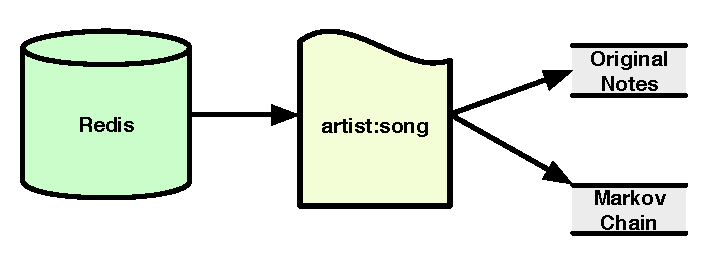
\includegraphics[width=.7\linewidth]{Pictures/mongo_knowledge_base.pdf}}
\caption{Extracted MIDI Structure}
\label{fig:md_kb}
\end{figure}

A Stream is organized by parts where each part contains either a nested Stream or a Measure. A Measure is a dictionary of concurrent music features where each key is a Music21 object and each value is the available music feature at a certain time segment.   As a result, it is easy to extract and analyze specific features from the Stream, e.g. finding a song's melody from timestamp $x$
to $y$, harmony from timestamp $i$ to $j$, most common note in parts $m$ through $n$, etc.

%The music server is a continually growing music encyclopedia that stores a song's metadata and musical features. This means that any application using the API has access to a plethora of music data. The metadata is mainly used for organization and searching. The heart of this server is in the corpus storage. Instant access to a song's corpus provides a variety of uses, e.g. song visualizations, or statistical analysis. A more detailed listing on available song features can be seen in Figure N. \\
%\\
%Currently, the API only supports GET, POST, and PUT requests. However, these are sufficient for the current capabilities of the server. Any third party application can add new data to the music server, e.g. if a song isn’t already in there it can easily be added. The music server is simply an expanding knowledge base that can be used for a multitude of musical applications. \\
%\\
%The music server can interact with any client capable of sending and receiving HTTP. Once the client sends the HTTP request with the desired parameters, the MIDI file is processed using music21, a Python library for music analysis from MIT. \\
%\\

\subsection{Breakdown of Interactive Genetic Algorithm}
\subsubsection{Initialization Settings}
The user is responsible for determining the initialization settings of the IGA. This is done by presenting the user with an initialization web-page and requiring all the form fields, which represent the required settings, to be filled out before the IGA can begin. These fields include: the influencer, the Markov chain size, the Markov chain history size, the number of notes per melody, the population size, the number of generations, and the mutation rate. This is can be seen in Figure~\ref{fig:index_ui}. 

%The user is responsible for determining the GA settings.The user is presented with a GA initialization form. The user determines what song will be used for influencing the initial population, the number of notes per melody, the population size, and the number of generations. This is shown in Figure~\ref{fig:index_ui}. 

\begin{figure}[H]
\center{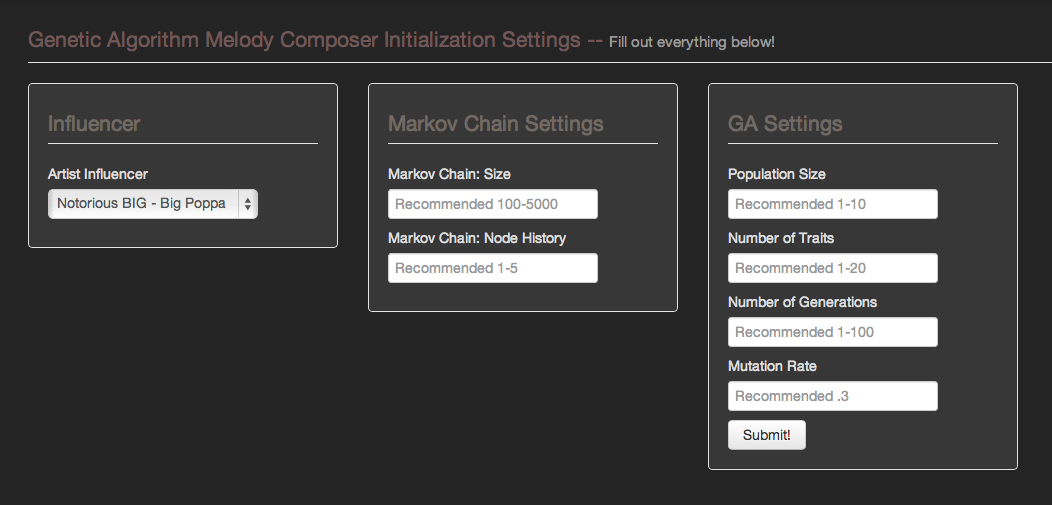
\includegraphics[width=1\linewidth]{Pictures/index_ui_small.png}}
\caption{Initialization Settings}
\label{fig:index_ui}
\end{figure}

\subsubsection{Influencer}
The influencer's role is to provide the IGA with structure and guidance when picking individuals from the search domain. This is a crucial component because it impacts the number of noisy individuals typically found in the initial population. \\
\\
%The search domain represents the set of possible individuals, i.e. the gene pool, that the GA pulls from to generate the initial population. The role of the influencer is to decrease the number of noisy individuals found in the initial population. This is done by providing the GA with structure and guidance when picking from the search domain. \\
%\\
%An influencer is used to generate the search domain. It provides the GA with structure and guidance when generating the initial population. The reason why it’s an important component is because of how it generates the search domain, which is essentially the gene pool that the GA is pulling from to generate the initial population. \\
%\\
Suppose that the search domain is generated randomly and individuals are also picked at random. For example, imagine that the search domain, $S$, only contains $[[A],[B,C,D],[E]]$ where a single element in a nested list represents a note and multiple elements in a nested list represent a chord. If an individual is an array of size 2 containing any combination of elements in $S$, possible solutions include, but are not limited to $[[A], [A]]$, $[[A], [B, C, D]]$, or $[[B, C, D], [E]]$. The immediate problem is that there’s no order or understanding of how to go about picking solutions; it is a free-for-all. This isn’t much of an issue when dealing with an automatic fitness function because the IGA has more time to evolve and filter out the noise due to the increased number of generations. However, this is not as simple when using an interactive fitness function because the number of generations are limited due to user burnout. As a result, earlier generations have a greater influence on individuals in later generations. \\

\\
Now, consider a search domain that is still generated randomly, but uses a rule-set to pick individuals, e.g. restricting the possible combinations to only allow major chords. Even if the rule-set is simple, the added structure yields better individuals because there's now a pattern to picking. However, this research is interested in generating melodies relevant to the user's musical taste, not on technical correctness. Such a rule-set would need to be generated dynamically in order to incorporate the user's preferences. The required rule-set to do this would be extremely complex making this an unattractive possibility. \\
\\
To solve this problem, a Markov chain is used to generate the search domain. It eliminates the need to embed rule-sets in the software and also provides the IGA with a search domain that represents the user's music preferences. In other words, the search domain is no longer polluted with random noise, and instead contains relevant data. This is similar to using a Markov chain to write sentences where the sentence may not make complete sense, but grammar, sentence structure, and dialogue from the original text will be followed to a degree \cite{website:rose}. By setting a prefix size, a model can be built by gathering statistics about the frequency of which words follow certain prefix groups of other words \cite{website:rose}. For example, if $n$=2, the next generated words are based on the previous two words. When applied to music, this results in new melodies that contain the style and hints of the original. \\
\\

Once the Markov chain generates a search domain, the IGA must create a pool of individuals for the initial population. In this instance, individuals can be created using random sampling or random continuous sampling. A random sampling is when random elements are selected from a list, e.g. if the search domain, $S$, only contains notes $[[C, C, A], [B, C, D], [A, B], [C\#, D], [A4, B5], [C6]]$ and an individual is an array of size 3, then a possible solution would be $[[A,  B], [C6], [A, B]]$ or $[[A, B], [A, B], [A, B]]$. However, this process essentially negates the work of the Markov chain because all it is doing is dynamically restricting the type of notes available in the search domain. Instead, random continuous sampling is used because it ensures that the Markov chain output is used correctly and it also adds a level of diversity to the population. Random samples are still taken from the search domain, but instead of randomly picking a single element, a consecutive series of elements are picked, e.g. $[[C, C, A], [B, C, D], [A, B]]$ or $[[C\#, D], [A4, B5], [C6]]$. An important question is how much impact replacement has on the initial population, i.e. should a series of notes be discarded from the pool once picked? This is concept is known as independent vs. dependent events.

\subsubsection{Markov chain Workflow}
%The user sets the Markov chain constraints on the types of traits available to the initial population. 
First, the user is responsible for both selecting an influencer from the list of available songs and setting the Markov chain constraints $size$ and $order$. The Markov chain $size$ represents the number of requested notes and the $order$ is the desired number of states. The requested song is then sent to the music server where the title is used to find the song's corpus. Once the corpus is found, the notes are extracted and used to genereate a $N^{th}$ order Markov chain. The Markov chain is then cached in redis as a hash set. Next, the IGA uses random sampling to generate the initial population.

%The MIDI server then extracts a subset of notes based on the population size and number of traits, and responds to the GA Server's request with a JSON object. 

%The user will be in control of the Markov chain constraints, $total\_size$ and $history\_size$. \\

\subsubsection{Evaluation}
The goal of this fitness function is two fold; improve the UX and improve the type of feedback. These factors are responsible for user burnout and the rate of evolution. The rate of evolution determines how well the current generation has evolved from the previous and can be measured by comparing the average fitness score between the $N^{th}-1$ generation and $N^{th}-2$ generation. In this IGA, 0 is the best score an individual can receive, thus it is important that the average fitness score of the current generation is closer to 0 than the previous generation's.
\\
The Euclidean distance, as seen in (\ref{ed}), is a technique used to determine the distance between 2 vectors, $p$ and $q$. 

\begin{equation}
	d(\textbf{p,q}) = \sqrt{\sum_{i=1}^n (q_i - p_i)^2} 
	\label{ed}
\end{equation}

The IGA uses this to calculate an individual's fitness score by finding the amount of change that has occurred between the original melody, $p$, and the adjusted melody, $q$. The amount of change is determined by comparing the index locations of the notes in the original melody with the index locations of the notes in the adjusted melody. In order to do this, the note's original index location as well as the note's value are stored in a list of tuples as $[(idx_{0},note_{0}), ... , (idx_{n}, note_{n})]$. If the user swaps the first note with the second note, then the index of the first item in the adjusted melody list will have an index of 1, while the index of the second item in the adjusted melody list will have an index of 0. An example can be seen in Figure~\ref{fig:ed_ex}. Additionally, there needs to be a limit on the number of adjustments the user can make to ensure that the fitness scores aren't all over the place. Currently, the number of allowed adjustments are 30\% of the total number of notes. Decimals less than 5 are rounded down, and decimals greater than 4 are rounded up.  For example, if a melody contains 10 notes, then the user can only make 3 changes (30\% of 10 = 3). \\

%The maximum fitness score is dependent upon the number of notes in an individual, but the range is always between 0 and $max(distance(p,q))$ where 0 is the desired score. Additionally, there needs to be a limit on the number of adjustments the user can make to ensure that the fitness scores aren’t all over the place. Currently, the number of allowed adjustments are 30\% of the total number of notes. Decimals less than 5 are rounded down, and decimals greater than 4 are rounded up.  For example, if a melody contains 10 notes, then the user can only make 3 changes (30\% of 10 = 3). \\

%In this research, it is used by the fitness function to calculate an individual's fitness score by determining the amount of change that has occurred between the original melody, $p$, and the adjusted one, $q$. \\


\begin{figure}[H]
\center{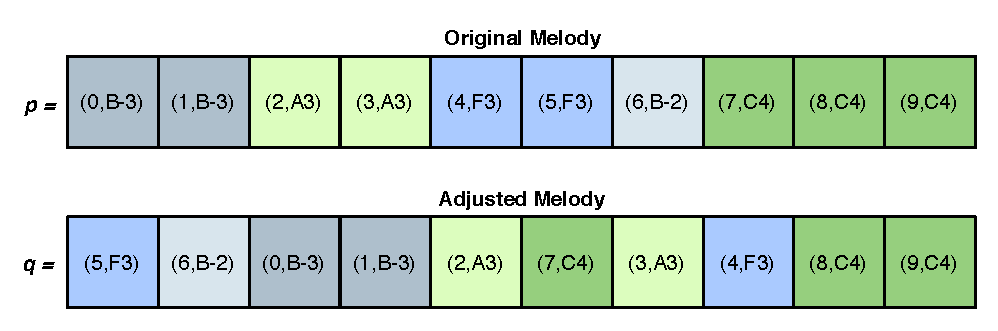
\includegraphics[width=1\linewidth]{Pictures/euclid_dist.pdf}}
\caption{Euclidean Distance}
\label{fig:ed_ex}
\end{figure}

Based on the individual in Figure~\ref{fig:ed_ex}, the maximum number of allowed adjustments are 3 since there are 10 notes, the fitness score is 24, and the pairs used to calculate the Euclidean distance can be seen in Table~\ref{tab:ed_coords}.
\begin{center}
\captionof{table}{Euclidean Distance Coordinates} \label{tab:ed_coords} 
%\begin{table}
    \begin{tabular}{|l|l|}
        \hline
        (0,5) & (1,6) \\ \hline
        (2,0) & (3,1) \\ \hline
        (4,2) & (5,7) \\ \hline
        (6,3) & (7,4) \\ \hline
        (8,8) & (9,9) \\ \hline
%        \hline
    \end{tabular}
%\end{table}
\end{center}
%In order to calculate the correctSmall changes, e.g. moving a note 1 spot from the original location, on an average sized individual, e.g. containing roughly 10 notes, will result in a very small Euclidean distance. However, gradually increasing the number of adjustments causes the Euclidean distance to significantly increase, as demonstrated in examples (\ref{ed_1}, \ref{ed_2}, \ref{ed_3}). 
%
%
%\begin{align}
%  &\begin{aligned}
%    p &= [A,B,C,D,A,E,B,D,C,F]\\ 
%    q &= [A,B,C,A,B,E,A,C,D,D] \\     
%      & Euclidean Distance(p,q) = 18 \\
%	\label{ed_1}
%  \end{aligned}\\
%  &\begin{aligned}
%    p &= [A,B,C,D,A,E,B,D,C,F]\\
%	q &= [D,C,B,A,A,E,B,D,C,F]\\
%	& EuclideanDistance(p,q) = 36 \\
%	\label{ed_2}
%  \end{aligned} \\
% &\begin{aligned}
%    p &= [A,B,C,D,A,E,B,D,C,F] \\
%	q &= [D,C,B,A,E,A,B,D,C,F]\\
%	& EuclideanDistance(p,q) = 46
%	\label{ed_3}
%  \end{aligned}	
%\end{align}
%\\
%\\
%Listening to a melody and ranking it based on some scale, e.g. 1-10, only tells the system how much the user liked the melody compared to the other melodies. It doesn't, however, say what the user liked or didn't like about the melody. Allowing the user to rate individual traits gives the system slightly more information about how the user liked the ordering of the pitches. However, in doing the above, the system still doesn't know what changes the user would have liked to see without doing heavy analysis on the placement of previous traits. In order to solve this, the fitness function in this research allows the user to re-order the pitches in a melody. As a result, the GA easily knows how much the user liked or disliked the original melody as well as what changes the user wants made. \\
%This adds a new level of functionality, and with further work will allow deeper analysis of what characteristics the user is looking for in a melody. \\

%$$\textrm{If } u=[A,B,C,D,A,E,B,D,C,F] \textrm{ and } v=[A,B,C,A,B,E,A,C,D,D], \textrm{ then the fitness score = } 18$$ $$
%\textrm{If } u=[A,B,C,D,A,E,B,D,C,F] \textrm{ and  } v=[D,C,B,A,A,E,B,D,C,F], \textrm{ then the fitness score = } 36$$ 
%$$\textrm{If } u=[A,B,C,D,A,E,B,D,C,F] \textrm{ and  } v=[D,C,B,A,E,A,B,D,C,F], \textrm{ then the fitness score = } 46$$\\
%\\

%$$\textrm{If } u=[A,B,C,D,A,E,B,D,C,F] \textrm{ and } v=[A,B,C,A,B,E,A,C,D,D], \textrm{ then the fitness score = } 18$$ $$\textrm{If } u=[A,B,C,D,A,E,B,D,C,F] \textrm{ and  } v=[D,C,B,A,A,E,B,D,C,F], \textrm{ then the fitness score = } 36$$ $$\textrm{If } u=[A,B,C,D,A,E,B,D,C,F] \textrm{ and  } v=[D,C,B,A,E,A,B,D,C,F], \textrm{ then the fitness score = } 46$$\\
%\\
%A Euclidean distance of 0, meaning the user didn't make any changes, results in an ideal melody. However, if the Euclidean distance is large, meaning the user made the maximum number of changes, then the user's melody will be passed to the next generation as is. The benefit to this approach is that the IGA is always getting useful user feedback and rarely needs to scrap an individual. The only time a melody will be scraped is if it contains a single type of note, e.g. [B, B, B, B, B, B, B, B, B]. \\
%\\
User burnout is inevitable, but the onset of it is directly influenced by the quality of the UX, i.e. how engaging the process is. Typically, an IGA requires the user to examine each individual and assign it a score, i.e. the user listens to the melody and then provides a score representing how the melody was as a whole. An important question this approach raises is what happens if the user really liked parts of the melody, but as a whole didn't enjoy it? Assuming that the user provided a low fitness score the good parts will end up getting lost. This is an issue because it decreases the chance that future individuals will see the traits the user liked. A remedy for this is to modify the type of feedback that is supplied. However, before that can be done, the common approaches need to be analyzed. \\
\\
Suppose a population contains 5 individuals and runs for 5 generations. That means the user has to listen and evaluate 25 individuals. As a comparison, it is not uncommon for a GA using an automatic fitness function to contain hundreds of individuals and run for thousands of generations. Typically, the user assigns a fitness score through either a textbox, a slider, or pressing a “good” or “bad” button \cite{Biles94}. The last approach requires the least amount of physical work from the user, but results in slower rates of evolution because the fitness score is binary. The user either liked it, or didn't like it. \\
\\
Instead of using binary evaluation to assign an entire individual a score, suppose the user could assign scores to sub-segments of the individual, e.g. the user may have liked the first $x$ notes and the last $y$ notes, but hated everything in-between. In addition to introducing a variety of possible fitness scores, i.e. scores are no longer just 0 or 100, the IGA is also receiving meaningful feedback; the user is basically able to say what segments were liked and disliked. This concept was introduced by Biles for GenJam \cite{Biles94} and allows the user to listen to and see the melody evolve in real-time. Doing this requires the population to be modeled differently, though. Instead of a population consisting of $n$ individuals, GenJam's populations consist of a single, continuous individual. \\
\\
As demonstrated by Biles in GenJam, there is a strong connection between the UX and the type of feedback supplied \cite{Biles94}. However, instead of having the user listen and say "yes, I like this", "no, I don't like this", I believe that the user should be able to demonstrate how the melody should be structured. This lets the user simultaneously evaluate and mutate the individual, allowing the user to become a temporary composer. The user listens to the melody and makes adjustments to the note order. Once the user submits the melody, the Euclidean distance between the original and adjusted melody is taken. So, if the user liked the melody as is, then the fitness score becomes 0 since no changes were made. This type of feedback also enhances the rate of evolution because the adjustments, if any, overwrite the original melody.  If the adjusted individual ends up getting picked during the selection process, then the child it creates will contain properties the user likes, which wouldn't happen if the adjustments didn't overwrite the original. \\
% An important consideration is that even a signle note out of place can throw off the whole melody. So, I basically allow the user to make these fixes. An important question to ask is how many changes can the user make? \\
\\
%There needs to be a limit on the number of adjustments the user can make to ensure that the fitness scores aren’t all over the place. Currently, the number of allowed adjustments are 30\% of the total number of notes. Decimals less than 5 are rounded down, and decimals greater than 4 are rounded up.  For example, if a melody contains 10 notes, then the user can only make 3 changes (30\% of 10 = 3). \\
%\\
Ideally, the IGA will produce a melody that requires the user to make no changes. However, suppose that the melody is horrible sounding, but the user is able to salvage it by making adjustments, and once the adjustments are made the user actually really likes the way the newly adjusted melody sounds. In this instance, the fitness score would be relatively high (based on the number of adjustments made), and thus this individual would have an extremely small chance of being picked during tournament selection. To account for this, the user is able to override the fitness score and reduce it in order to increase the probability that it gets selected. The number of times the user can do this per generation is limited and based on the number of individuals in the current generation. \\
\\
In addition to the auditory component, the fitness function also contains a visual component. Each note in the melody is a different color. Notes with the same pitch, but different octaves and accidentals are a different shade of the base color, e.g. if an individual contains [...,C, C\#4, C8,...] and C is green, then C\#4 might be light green and C8 might be dark green. This is done for both aesthetics and learning. It allows the user to pick up on visual patterns that may occur across individuals. An additional feature is that whenever the user makes an adjustment, the fitness score is immediately updated and displayed in the stats widget. This is so the user can see the impact the adjustment has on the score.\\
\\
The key components this fitness function improves on are the type of feedback and the UX. Allowing the user to make adjustments provides more meaningful feedback because the fitness score is not calculated by how much the user liked the individual, but by how the user would have structured the melody given the same notes. Allowing the user to act as a composer builds on the overall experience because the user has a sense of ownership and can see how the adjustments impact future generations. Additionally, being able to experiment with music provides a fun factor. The fitness function is essentially providing the user with a template or a suggested melody, and allows users, even ones with no musical knowledge, to experiment and learn about music in a very straightforward, non-overwhelming way. An example of the fitness function can be seen in Figure~\ref{fig:fitness_ui}.

\begin{figure}[H]
\center{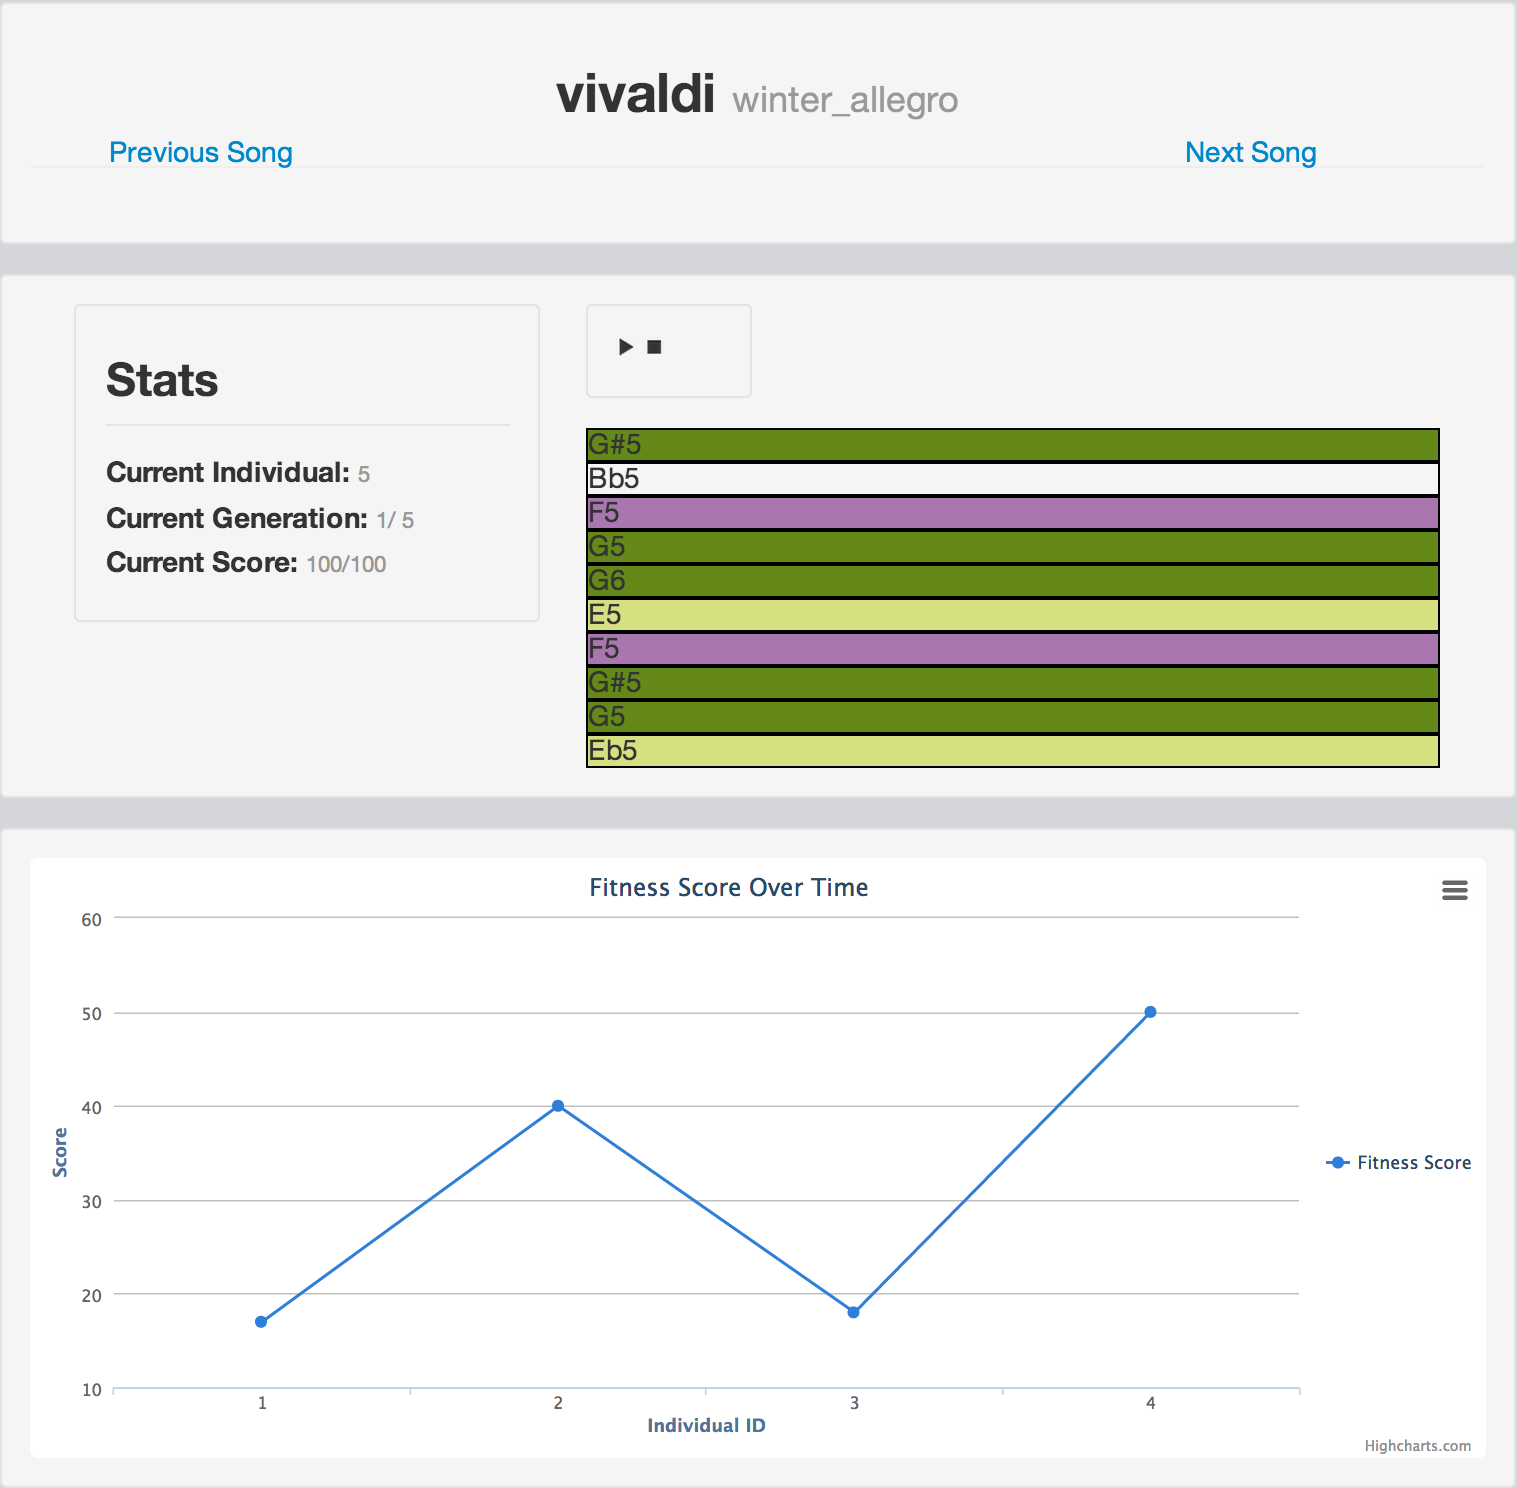
\includegraphics[width=.7\linewidth]{Pictures/fitness_ui.png}}
\caption{Fitness UI}
\label{fig:fitness_ui}
\end{figure}

\subsubsection{Fitness Workflow}
The user listens to a melody and either likes it as is and moves on to the next one, or doesn't like it. In the former, the melody is given a fitness score of 0, meaning that it was perfect; the user really liked it. In the latter, the user can make a change and preview it. The user can take as much time as needed to make adjustments to the melody; the only constraint is the number of allowed adjustments. The user can listen to the melody at any time by clicking the “Play” button allowing the user to hear how the adjustments sound. The user is also able to revert back to the original, pre-adjusted, melody if the adjustments aren't liked. 

\subsubsection{Genotype}
Typically, genotypes are encoded in either string or binary format because it's easy to store, process, and is fast. However, this project encodes an indivudal's genotype as a python dictionary making it easy to send as JSON and store in redis hash sets. \\
\\
The dictionary contains a set of keys representing an individual's metadata. Because this project focuses on generating melodies, many musical features can be ignored since a melody is a combination of notes, rests, and a duration. A note is a 1:1 mapping to a frequency and is made up of three components: a pitch, an accidental, and an octave.  The pitch is the degree of the tone, i.e. how high or low the frequency is, and is represented by letters A-G. An accidental is optional and is denoted by either $\#$ or $\flat$. It raises or lowers the key signature of a pitch. An octave is represented by an integer $0-9$ and is the "interval between one musical pitch and another with half or double its frequency" \cite{website:wiki_octave}. One modification has been made to the representation of a melody. Instead of a melody containing a list of notes, the melody contains a list of lists, where each sub-list can either be a single note, or a chord, e.g.

$\left\{\right
	score: 0, id: 1, generation: 1, notes: [[A, B, C], [B], [D, D, D]] 
\}$ \\

\\
A note is formed once the components are combined, which can then be converted to its respective frequency, and listened to. "Any note is an integer of half-steps away from middle A (A4) where the distance is denoted by $n$. If the note is above A4, then $n$ is positive; if it is below A4, then $n$ is negative. For example, one can find the frequency of C5, the first C above A4. There are 3 half-steps between A4 and C5 (A4 $\rightarrow$ A\#4 $\rightarrow$ B4 $\rightarrow$ C5), and the note is above A4, so n = +3" \cite{website:wiki_note}. As a result, the frequency of C5 is roughly 523.2Hz when calculated using the equation found in (\ref{note_to_freq}).

\begin{equation}
	f = 2^{n/12} \cdot 440Hz
	\label{note_to_freq}
\end{equation}
\\
\subsubsection{Genetic Mapping}
Genetic mapping transforms the genotype into a phenotype, which means taking a series of notes and turning them into a melody that the user can listen to. In this instance, the genotype is a list of dictionaries and the phenotype is a melody. \\%is a list of tuples with a frequency and duration. \\
%Each dictionary contains the pitch, accidental, octave, and duration.\\
\\
Mapping the genotype to the phenotype is done by first, searching through the list of dictionaries. For each dictionary, the notes key is extracted and for each note in the list of notes, the pitch frequency is generated and stored in a tuple. \\

This process is performed on the client's machine using JavaScript. The IGA sends the browser the genotype encoded as a JSON object containing a list of dictionaries. Each note is displayed in its own div element on a HTML page where the div ID is set to the note's value, e.g. div id="C5". Whenever the user makes an adjustment and wants to hear it, the JavaScript reads the div elements in order, converts each note to its frequency, and outputs the audio in the browser using the web-audio API.%\\
%\\
%A bottleneck occurs if the user makes a lot of adjustments. Re-calculating the frequency whenever an adjustment is made results in a 3-5 second gap from the time the user presses the “Play” button until the sound can be heard. To remove this gap, the frequency for each of the notes is calculated at startup and stored in a dictionary. In JavaScript that means storing the frequencies in JavaScript objects; an entity that contains properties and types. The property is the note (div ID) and the type is the frequency. Using objects reduces the complexity to O(1) because the property is already known resulting in an instant lookup.

\subsubsection{Interactive Genetic Algorithm Operators}
IGA operators are done server-side using Python. This includes selection, crossover, and mutation.\\
\\
%The IGA uses tournament selection to generate a mating pool by randomly selecting $k$ individuals from the current generation. The selected individuals are sorted by their fitness score in ascending order and the $j$ individuals with the lowest fitness score are selected for the mating pool. This process is repeated $n$ times. In order for the user adjusted melodies to have a chance at being picked, it is imperative that $k$ is smaller than $n$. As a result, the size of $n$ is set to ceiling($k$ $\cdot$ 1.5), e.g. if $k$ = 3 then $n$ = 5. This is because higher fitness scores don't always mean that the individual should be trashed. By keeping $k$ small and $n$ large, the IGA doesn't ignore the user adjusted melodies. On the contrary, if $k$ is large and $n$ is small then the individuals with high fitness scores will be overlooked. \\
The IGA uses tournament selection to decide which individuals will be selected for crossover by randomly selecting $k$, the tournament size, individuals from the current population. The individual with the best (lowest) fitness score is picked and placed in the crossover pool. There are $n$ rounds in a tournament and the process allows for an already selected individual to be picked again, i.e. independent events. An example can be seen in Figure~\ref{fig:selection_ex}.

\begin{figure}[H]
\center{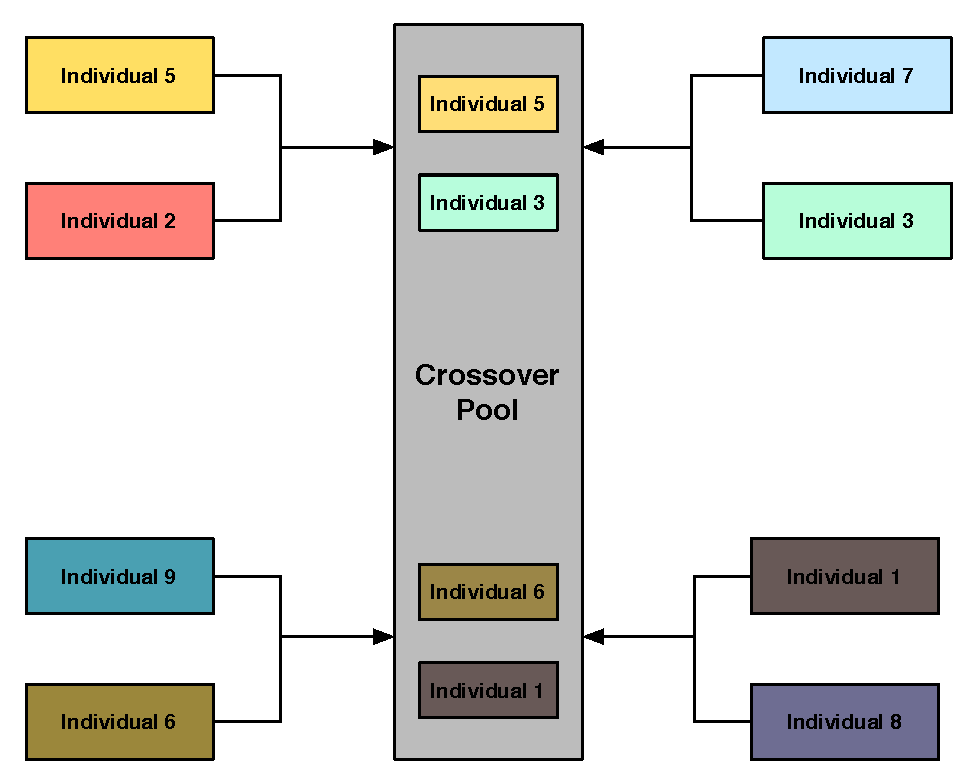
\includegraphics[width=.7\linewidth]{Pictures/selection.pdf}}
\caption{Selection: $k$=2, $n$=4}
\label{fig:selection_ex}
\end{figure}

It is possible to modify the probability of weaker individuals (higher fitness scores) being picked by adjusting $k$. Each increment of $k$ increases the probability of selecting only the best individuals from the population, while decrementing $k$ increases the probability of selecting weaker individuals from the population, i.e. as $k$ grows or shrinks so does the probability of selecting certain types of individuals.  In this research, some good individuals may exist in the population with a weak fitness score, thus $k$ will be set to 2 resulting in binary tournament selection during each round, $n$. The value of $n$ determines the size of the next generation's population. In order for the population size to remain consistent from generation to generation, $n = \frac{1}{2} * p$ where $p$ is the population size. In order to account for the other half of the population, each iteration of crossover yields 2 children. The general algorithm can be seen in Algorithm~\ref{algo:select}.

\begin{algorithm}[H]
$counter$ = 0\;
\While{counter \textless N} {
	Randomly select $k$ individuals from the current generation\;
	Select the individual with the lower fitness score and add it to the crossover pool\;
}
 \caption{Selection Algorithm}
\label{algo:select}
\end{algorithm}

%\begin{itemize}
%\item Loop $n$ times
%	\begin{itemize}
%	\item Randomly select $k$ individuals from the current generation
%	\item Select the individual with the lower fitness score and add it to the crossover pool
%	\end{itemize}
%\end{itemize}

Once the selection process has been completed, the IGA undergoes crossover and creates the next generation of individuals. The IGA uses single point crossover yielding two new children per iteration. First, two parents are randomly selected from the crossover pool. A random split point is generated to determine what traits from which parent the child will be made up of. An example can be seen in Figure~\ref{fig:crossover_ex}.

\begin{figure}[H]
\center{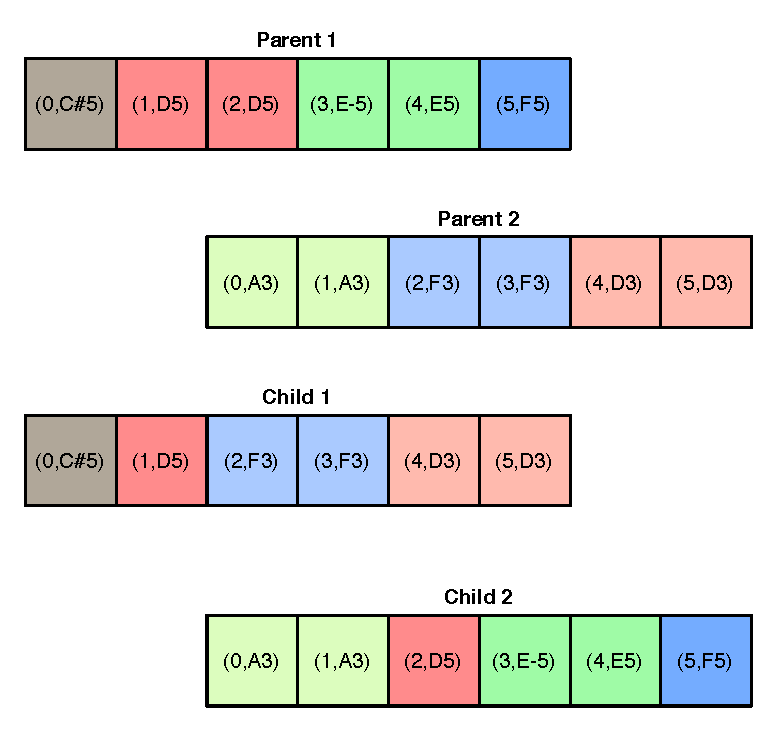
\includegraphics[width=.7\linewidth]{Pictures/crossover.pdf}}
\caption{Crossover: $split point$=2}
\label{fig:crossover_ex}
\end{figure}

There is a 50\% chance that there will be an odd number of parents in the crossover pool. If $n$ is an odd number then one parent will have to crossover twice resulting in some commonalities among 4 individuals of the next generation. However, since the crossover point is randomly selected this will not be much of an issue. For this reason, it is important to keep track of which individuals crossover with each other to ensure that there are no duplicates, otherwise there is a chance that the same two individuals might crossover with each other twice. To account for this, parents are stored in a tuple with the lower parent id always being at index 0 in the tuple. Each pair is then appended to a set to ensure that there are no duplicates. \\
\\
After crossover is complete and the next generation has been created, it is necessary to mutate random individuals in order to diversify the population. The mutation rate, $m$, is a decimal between $[0,1]$ that is decided upon during the IGA's initialization. For each individual in the population, a random decimal $n$ between $[0,1]$ is also generated. If $n > m$ then the current individual undergoes mutation. A random mutation point, $rmp$ between $[0, individualSize]$, and a random range, $rr$ between $[rmp,individualSize]$ are generated to determine which notes will be mutated. A new Markov chain is then created using the same influencer, and a subset of consecutive notes in the Markov chain are used to replace the notes in individual's mutation range. The general algorithm can be seen in Algorithm~\ref{algo:mutation}.

\begin{algorithm}[H]
$mutationRate$ = .3\;
\For{each individual}{
	$rnd$ = randomDecimal(0, 1)\;
	\If{rnd $\textgreater$ mutationRate}{
		$start, stop$ = randomSubset(individual)\;
		$newGenome$ = markovChain($start-stop$)\;
		$individual[start:stop]$ = $newGenome$\;
	}
}
 \caption{Mutation Algorithm}
\label{algo:mutation}
\end{algorithm}

%\begin{itemize}
%\item For each individual
%	\begin{itemize}
%	\item $n$ = random decimal	
%	\item If $n >$ mutation rate
%		\begin{itemize}
%		\item $rmp$ = mutation point
%		\item $rr$ = random subset
%		\item $k$ = random range betwenn 1 and size of individual
%		\item Generate Markov chain 
%		\item $j$ = $rr$ consecutive notes from Markov chain
%		\item Individual[$rmp$ : $rr$] = Individual[$j$]
%		\end{itemize}
%	\end{itemize}
%\end{itemize}

%TALK ABOUT MARKOV CHAIN AND MUTATION! The IGA utilizes mutation in a non-conventional fashion. Essentially, mutation happens in the fitness function if the user makes adjustments to the individual. These adjustments overwrite, or mutate the individual. This type of mutation occurs at a much earlier stage than traditional implementations. Typically if mutation occurs, it's on the child immediately after crossover. In this instance, it occurs during the fitness function. Because more than a few adjustments to an individual greatly impacts the fitness score, the probability that the adjusted individual is picked during selection greatly diminishes; much like having a low mutation rate results in a low probability of a child being picked for mutation.

\subsubsection{Interactive Genetic Algorithm Workflow}
The IGA workflow is extremely straightforward. The user is presented with a settings webpage, which is used to fill out the initialization parameters. These include: population size, number of traits, number of generations, mutation rate, Markov chain size, Markov chain node history, and the influencer. These parameters are processed and a request is sent to the music server. The music server then calls the GA with the users preferences. The GA generates the initial population and caches it in redis. Next, the user is presented with a web-page for the fitness function where the user evaluates each individual, one by one. After the user is satisfied with the individual, the fitness score is calculated by taking the Euclidean distance between the pre-adjusted melody and the post-adjusted melody. The fitness score and the adjusted melody are sent to the IGA with an AJAX request. Once an individual has been evaluated and sent back to the server, the GA needs to know how to proceed. Essentially, the GA needs to check if the termination requirements have been met. First, the GA checks to see if there are more individuals in the current generation that need to be evaluated. If there are, then the GA returns to the fitness function. If there aren't any more individuals, then the GA checks to see if there are any generations remaining. If there aren't, then the GA terminates, otherwise the GA moves onto selection, crossover, mutation, and then back to the fitness function where this whole process is repeated. The general workflow can be seen in Figure~\ref{fig:workflow}.

\begin{figure}[H]
\center{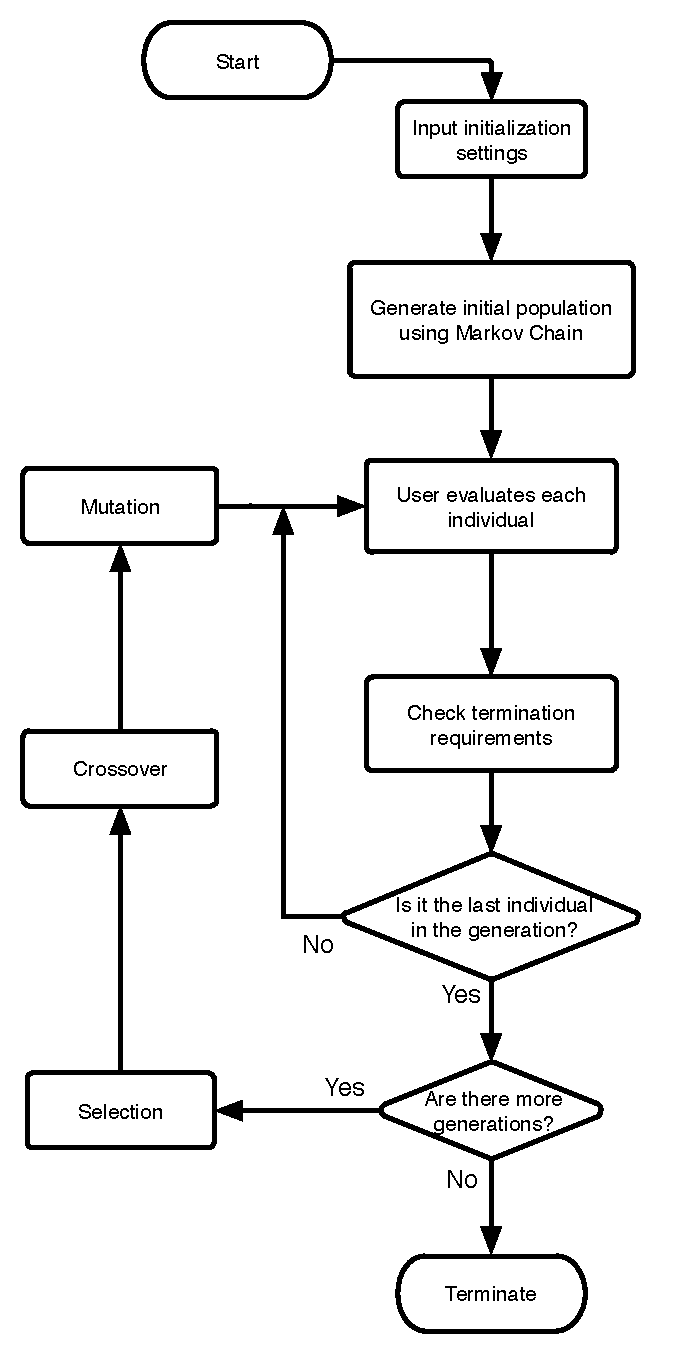
\includegraphics[width=.8\linewidth]{Pictures/workflow.pdf}}
\caption{General Workflow}
\label{fig:workflow}
\end{figure}

\section{Results}
\subsection{Overview}
Tests were designed around determining which combination of the initial population and fitness function yielded better individuals in the least amount of time. Each GA was initialized with the same settings, which can be seen in Table~\ref{tab:init_settings_results}.

\begin{center}
%\begin{table}
	\captionof{table}{Initialization Settings} \label{tab:init_settings_results} 
    \begin{tabular}{|l|l|}
        \hline
	\bf{Influencer}         & Antonio Vivaldi - Winter: Allegro (Non Molto)\\ \hline
	\bf{Markov Chain Size}         & 2500 \\ \hline
	\bf{Markov Chain Node History} & 3    \\ \hline 
	\bf{Population Size}           & 5    \\ \hline
	\bf{Number of Notes}           & 10   \\ \hline 
	\bf{Number of Generations}     & 5    \\ \hline 
	\bf{Mutation Rate}             & .3   \\ \hline
%        \hline
    \end{tabular}
%\end{table}
\end{center}

\subsection{Test 1: Random Population and User Scoring}
\begin{figure}[H]
\center{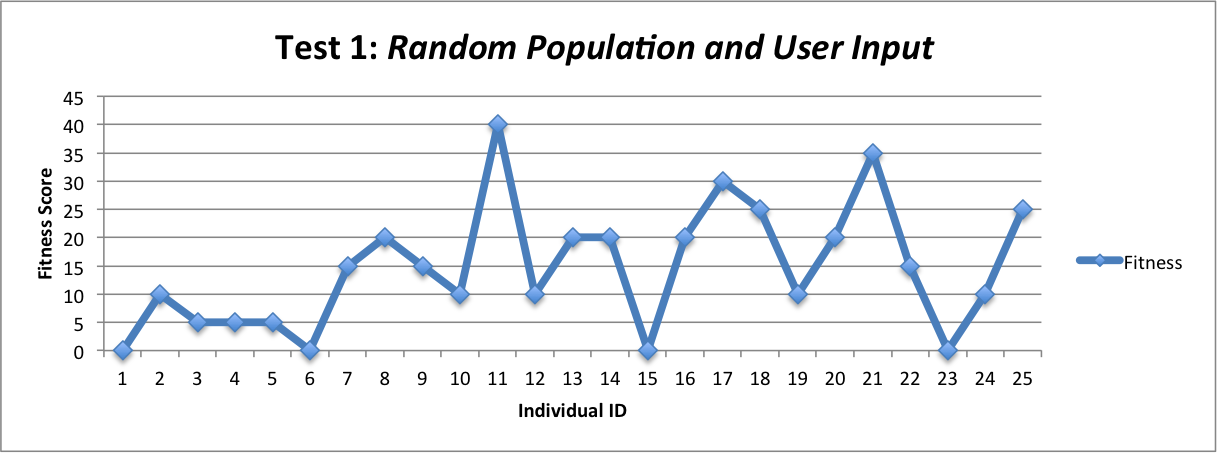
\includegraphics[width=.8\linewidth]{results/test1.png}}
\caption{Test 1: Random Population and User Scoring}
\label{fig:test1}
\end{figure}
\begin{center}
	\captionof{table}{Fitness Score Stats for Test 1} \label{tab:stats_t1} 
    \begin{tabular}{|l|l|}
        \hline
	\bf{Mean}         & 14.6\\ \hline
	\bf{Median}         & 15 \\ \hline
	\bf{Best} & 4\\ \hline 
    \end{tabular}
\end{center}
This combination generated terrible sounding individuals. The minimal number of generations in conjunction with an unintelligent seed function produced results comparable with someone hitting random keys on a piano. This was to be expected, though. The leading issue with this combination was the number of generations. 5 generations did not provide enough time for all of the poor individuals typically found in the beginning to die off. Additionally, this combination lacks chromosome repair so there was no way for the user to influence an individual. As a result, the growth of individuals was extremely slow, unstructured, and often regressed from generation to generation. User fatigue was minimal, although users reported boredom due to lack of interesting melodies and repetitive nature of the fitness function. User never found a "favorite" melody and considered them to all be of poor quality. \\

\subsection{Test 2: Random Population and Trait Re-ordering with Euclidean Distance}
\begin{figure}[H]
\center{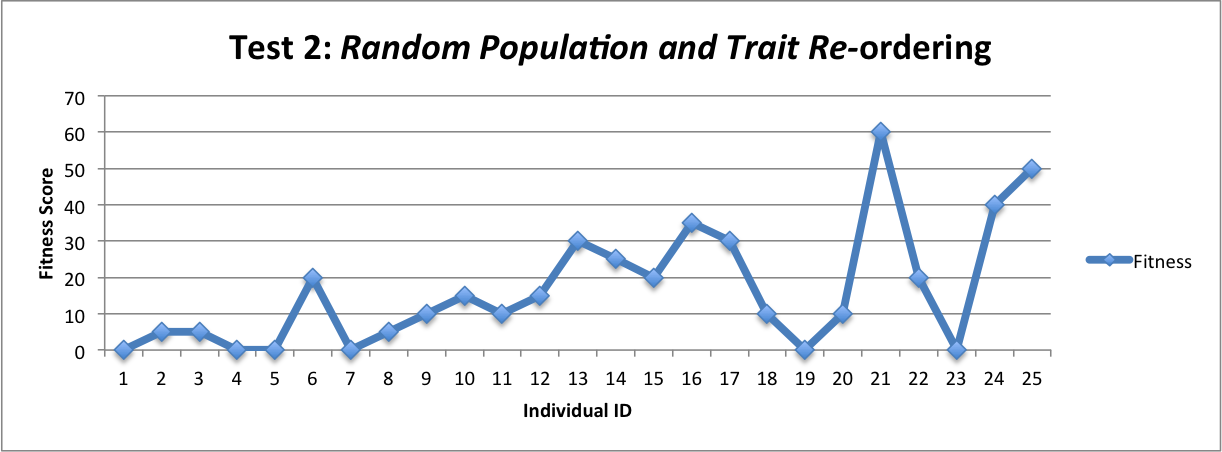
\includegraphics[width=.8\linewidth]{results/test2.png}}
\caption{Test 2: Random Population and Trait Re-ordering with Euclidean Distance}
\label{fig:test2}
\end{figure}
\begin{center}
	\captionof{table}{Fitness Score Stats for Test 2} \label{tab:stats_t2} 
    \begin{tabular}{|l|l|}
        \hline
	\bf{Mean}         & 16.6\\ \hline
	\bf{Median}         & 10 \\ \hline
	\bf{Best} & 60\\ \hline 
    \end{tabular}
\end{center}
This combination generated extremely poor individuals in the first generation due to using a random population, however this was quickly remedied in generation 2 due to chromosome repair, i.e. the user's ability to re-organize each individual. While the user made the maximum number of re-orderings allowed per individual, the user was still able to make part of the individual have a funky/fun sound. This can be attributed to the fact that the random population provided a large spectrum of possible notes per individual allowing the user to create interesting patterns. As a result, the growth of individuals started off slowly, but quickly sped up and produced much more interesting melodies in later generations due to the user's help. Additionally, the user was less bored because the user felt more involved in the process. The user reported that boredom and fatigue began to set in during generations 4 and 5 because it began to get very tedious and repetitive. It also took a while for the user to find a favorite melody. \\

\subsection{Test 3: Markov Chain and User Scoring}
\begin{figure}[H]
\center{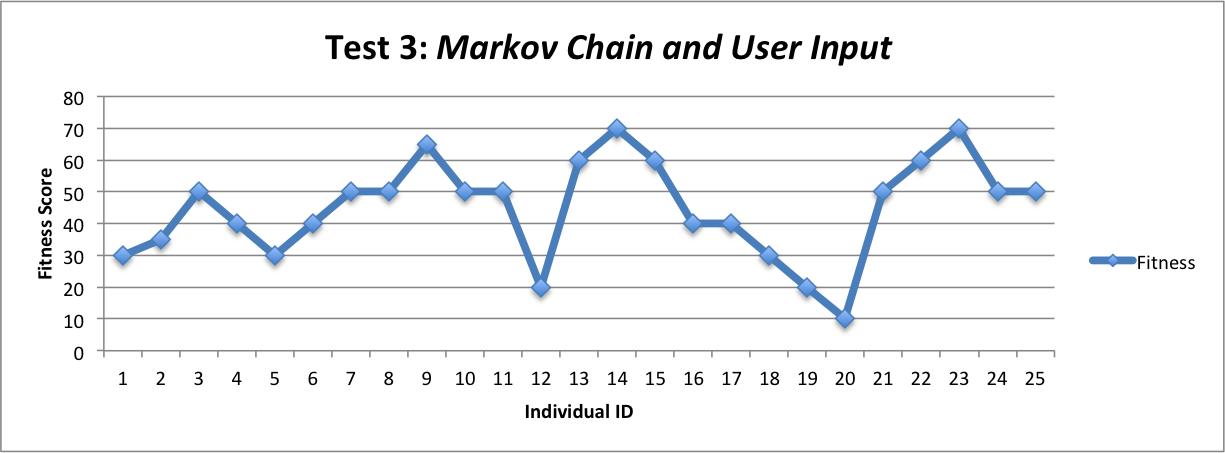
\includegraphics[width=.8\linewidth]{results/test3.png}}
\caption{Test 3: Markov Chain and User Scoring}
\label{fig:test3}
\end{figure}
\begin{center}
	\captionof{table}{Fitness Score Stats for Test 3} \label{tab:stats_t3} 
    \begin{tabular}{|l|l|}
        \hline
	\bf{Mean}         & 44.8\\ \hline
	\bf{Median}         & 50 \\ \hline
	\bf{Best} & 70\\ \hline 
    \end{tabular}
\end{center}

This combination provided decent results in earlier generations since the initial population was intelligently generated based off of a song the user already liked. In terms of individual growth from generation to generation, this test was comparable with test 4. The quality of each individual in generation 1 was much better than in tests 1 and 2. Additionally, the fitness score of the best individual grew significantly from generation to generation. The issue with this test was the lack of chromosome repair resulting in some pretty poor patterns.  User fatigue was minimal like in test 1, and it took longer for the fatigue and boredom to set in since the melodies produced were entertaining.\\

\subsection{Test 4: Markov Chain and Trait Re-ordering with Euclidean Distance}
\begin{figure}[H]
\center{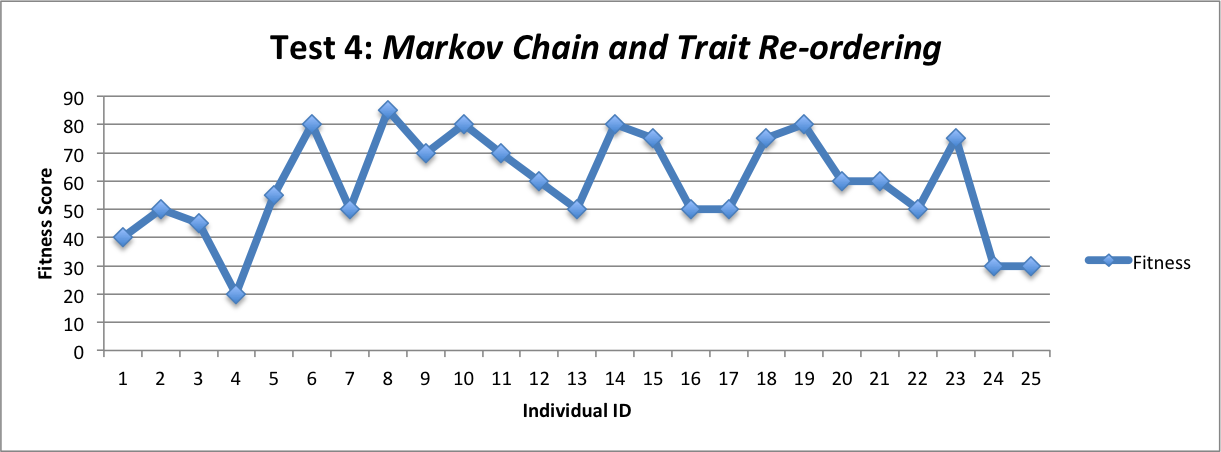
\includegraphics[width=.8\linewidth]{results/test4.png}}
\caption{Test 4: Markov Chain and Trait Re-ordering with Euclidean Distance}
\label{fig:test4}
\end{figure}
\begin{center}
	\captionof{table}{Fitness Score Stats for Test 4} \label{tab:stats_t4} 
    \begin{tabular}{|l|l|}
        \hline
	\bf{Mean}         & 58.8\\ \hline
	\bf{Median}         & 60 \\ \hline
	\bf{Best} & 85\\ \hline 
    \end{tabular}
\end{center}
This combination generated the best sounding individuals as well as reduced fatigue and boredom when compared to test 3. This can be attributed to the fitness function. It appears that a more involved fitness function reduces the onset of boredom and fatigue since the user feels more involved in the process. Additionally, most of the poor individuals were seeded out after the first generation. \\

\subsection{Analysis of Tests}
Tests 1 and 3 took less time to complete compared to tests 2 and 4. This was because it was much easier for the user to just enter a number in and click next opposed to re-arranging the traits. In contrast, the user had a much more enjoyable experience in tests 2 and 4 opposed to tests 1 and 3. The user felt involved in the process, and even compared it to solving a puzzle. As a result, the fatigue level was minimal for the first 3 generations in tests 2 and 4. The last 2 generations in tests 2 and 4 were much more tiring and difficult for the user to put in as much as effort as was done in the first 3 generations, which explains the slight dip in fitness scores. However, the user enjoyed test 4 more than test 3, and stated that it took longer for boredom and fatigue to set in since the evaluation process was much more enjoyable. The user did not enjoy tests 1 and 3 mainly because the evaluation process was boring.  \\

\section{Conclusion} 
This research has provided a lot of insight into what needs to be done to generate melodies using an IGA. Specifically, it showed how reducing the size of the search space and then intelligently drawing from it influences the quality of individuals found in the initial population. Additionally, the results provided insight into how a more detailed fitness function can help increase the quality and rate of growth of individuals from generation to generation. The goals of this project were met, however, there is still much work that can be done to further reduce user fatigue levels while also increasing the quality of individuals.  \\

%The graph in Figure~\ref{fig:r_biggie_.4} represents the fitness score over time with the initialization settings seen in Table~\ref{tab:r_biggie_4}. While the fitness scores appear to jump up and down, which may be attributed to the low population size, low number of generations, and moderate mutation rate, as a whole, the fitness scores do decrease over time.
%
%
%\begin{figure}[H]
%\center{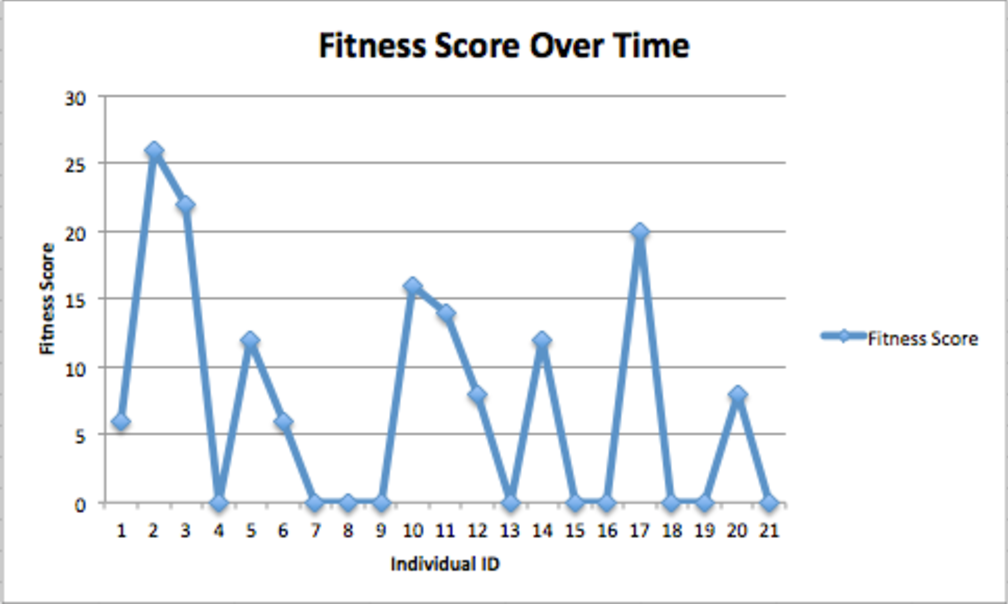
\includegraphics[width=.8\linewidth]{Pictures/graphs/biggie_3000_3_3_10_3_4.pdf}}
%\caption{Influencer: Notorious BIG - Big Poppa}
%\label{fig:r_biggie_.4}
%\end{figure}

%----------------------------------------------------------------------------------------
%	BIBLIOGRAPHY
%----------------------------------------------------------------------------------------
\bibliographystyle{plain}
\bibliography{Gelb-final-report}

%----------------------------------------------------------------------------------------

\end{document}
